\part{SW 03 - Präsentationen zu physikalischer Schicht}
\section{Lernziele (Leitfragen)}
\begin{itemize}
    \item Die physikalische Schicht und Zugriffsverfahren (T1)
    \begin{enumerate}
        \item Was ist der Zweck der physikalischen Schicht?
        \item Was sind die Hauptmerkmale der physikalischen Schicht?
        \item Was ist der Unterschied zwischen \flqq{}Simplex\frqq, \flqq{}half-duplex\frqq{} and \flqq{}full duplex\frqq?
        \item Welches sind die am häufigsten verwendeten Zugriffsverfahren?
        \item Was ist der Unterschied zwischen CSMA/CD und CSMA/CA? Wo werden sie verwendet?
        \item Was bedeutet „Late Collision“?
        \item Was muss man noch unbedingt über die physikalische Schicht und Zugriffsverfahren wissen?\\
    \end{enumerate}

    \item Topologien und ``Bandwidth'' (T2)
    \begin{enumerate}
        \item Was für Topologien findet man in Computernetzwerken?
        \item Wo ist der Unterschied zwischen \flqq{}Bandwidth\frqq, \flqq{}Throughput\frqq{} und \flqq{}Goodput\frqq? Wie kann man diese Konzepte visualisieren und verstehen?
        \item Was ist \flqq{}Latency\frqq{} und \flqq{}Jitter\frqq? Wie kann man diese Konzepte visualisieren und verstehen?
        \item Was muss man noch unbedingt über Topologien und ``Bandwidth'' wissen?\\
    \end{enumerate}

    \item Kupferkabel (T3)
    \begin{enumerate}
        \item Was sind die wichtigsten Merkmale von Kupferkabeln?
        \item Was für Kupferkabelarten werden heutzutage in Computernetzwerken am häufigsten verwendet?
        \begin{enumerate}
            \item Wie sind sie aufgebaut?
            \item Wie sehen die Stecker aus?
        \end{enumerate}
        \item Worauf muss bei der Handhabung und Verlegung der Kupferkabel besonders geachtet werden und warum?
        \item Woraus resultieren die Längenbeschränkungen der Kupferverkabelung?
        \item Was muss man noch unbedingt über Kupferkabel wissen?\\
    \end{enumerate}

    \item Glasfaserkabel (T4)
    \begin{enumerate}
        \item Was sind die wichtigsten Merkmale von Glasfaserkabeln?
        \begin{enumerate}
            \item Wie sind sie aufgebaut?
            \item Wie sehen die Stecker aus?
        \end{enumerate}
        \item Worauf muss bei der Handhabung und Verlegung von Glasfaserkabeln besonders geachtet werden und warum?
        \item Woraus resultieren die Längenbeschränkungen der Glasfaserkabelverkabelung?
        \item Wo ist der Unterschied zwischen Multi- und Singlemode (Monomode)- Glasfasern?
        \item Was sind die Vor- und Nachteile von Glasfaserkabel (im Vergleich zu Kupferkabeln)?
        \item Was muss man noch unbedingt über Glasfaserkabel wissen?\\
    \end{enumerate}

    \item Wireless Access (T5)
    \begin{enumerate}
        \item Was sind die wichtigsten Merkmale von \flqq{}Wireless Media\frqq?
        \item Welche Wireless Access Geräte arbeiten auf Layer I?
        \item Was für Wireless Standards gibt’s in Computernetzwerken?
        \begin{enumerate}
            \item Was sind ihre Hauptmerkmale und Anwendungsbereiche?
        \end{enumerate}
        \item Was sind die Vor- und Nachteile von \flqq{}Wireless Access\frqq{} Methoden im Vergleich mit \flqq{}Wired Access\frqq?
    \end{enumerate}
\end{itemize}

\section{Antworten T1}
\subsection*{Was ist der Zweck der physikalischen Schicht?}
\begin{itemize}
    \item Bietet elektrische, mechanische und funktionale Schnittstelle zum Medium
    \item Definiert die Grösse der Bits (Geschwindigkeit)
    \item Definiert die Art der Übertragung und Codierung (z.B. elektromagnetische Wellen)
    \item Kommunikation zwischen Übertragungsmedien
    \begin{itemize}
        \item Lichtwellenleiter
        \item Stromkabel
        \item Stromnetz
    \end{itemize}
\end{itemize}

\subsection*{Was sind die Hauptmerkmale der physikalischen Schicht?}\index{Schichten!Physikalicshe Schicht}
\begin{itemize}
    \item Digitale Bit-Übertragung: \textsl{funktioniert indem...}
    \begin{itemize}
        \item \textsl{\dots{}über Kabel\dots}
        \begin{itemize}
            \item Kupfer, Lichtwellenleiter, Stromnetz
        \end{itemize}
        \item \textsl{\dots{}eine Verbindung\dots}
        \begin{itemize}
            \item statisches Multiplexing (synchron)
            \item dynamisches Multiplexing (asynchron)
        \end{itemize}
        \item \textsl{\dots{}an die richtigen Steckplätze hergestellt wird.\dots}
    \end{itemize}
    \item Definition der Übertragung eines Bits
    \begin{itemize}
        \item Dabei nicht nur 0 oder 1, sondern mehr
        \begin{itemize}
            \item Lichtintensität (Glasfaser)
            \item Spannung \& Ströme (elektrische Leitung)
            \item Binär (Datenstrom)
        \end{itemize}
        \item Übertragungsart muss mit Codierung versehen werden
    \end{itemize}
\end{itemize}

\subsection*{Was ist der Unterschied zwischen \flqq{}Simplex\frqq, \flqq{}half-duplex\frqq{} and \flqq{}full duplex\frqq?}\index{Kommunikation!Simplex}\index{Kommunikation!Half-Duplex}\index{Kommunikation!Full-Duplex}\index{Simplex}\index{Half-Duplex}\index{Full-Duplex}
Vergleiche Kommunikationsrichtung, das Senden/Empfangen, Leistung und Beispiele:
\begin{itemize}
    \item Simplex
    \begin{itemize}
        \item Unidirektional
        \item Nur Sender schickt Daten
        \item Schlechteste Leistung in Übertragung
        \item Tastatur$\rightarrow$Monitor
    \end{itemize}
    \item Half-Duplex
    \begin{itemize}
        \item Bidirektional: eins auf einmal
        \item Sender kann Daten senden und empfangen, aber nur ein Sender auf einmal
        \item Besser als Simplex
        \item Walkie-Talkie
    \end{itemize}
    \item Full-Duplex
    \begin{itemize}
        \item Bidirektional: alle gleichzeitig
        \item Sender schickt und empfängt Daten gleichzeitig
        \item Beste Leistung
        \item Telefon
    \end{itemize}
\end{itemize}

\subsection*{Welches sind die am häufigsten verwendeten Zugriffsverfahren?}\index{Zugriffsverfahren}\index{CSMA - Carrier Sense Multiple Access}\index{Zugriffsverfahren!CSMA}\index{Nichtdeterministische Zugriffsverfahren}\index{Deterministische Zugriffsverfahren}
Es gibt zwei Oberbegriffe:
\begin{itemize}
    \item \textbf{Nichtdeterministischer/stochastische Zugriffsverfahren}
    \begin{itemize}
        \item Jeder Teilnehmer kann zu jedem Zeitpunkt einen Kanalzugriff versuchen
        \item Zuteilungszeitpunkt lässt sich nicht vorherberechnen
        \item Hohe Netzauslastung \& Wartezeiten
        \begin{itemize}
            \item CSMA/CD
            \item CSMA/CA
            \item (Siehe \underline{\hyperref[sub:csma]{nächste Frage}})
        \end{itemize}
    \end{itemize}
    \item \textbf{Deterministische Zugriffsverfahren (kontrollierter Zugriff)}
    \begin{itemize}
        \item Sender zu Beginn einer Datenübertragung eindeutig bestimmt
        \item Zeitpunkt des Buszugriffs kann vorhergesagt werden (wichtig für Echtzeitanwendungen)
        \begin{itemize}
            \item Token-Passing
            \item Multiplexing-Verfahren
            \item Polling
        \end{itemize}
    \end{itemize}
\end{itemize}

Heutzutage wird vor allem das \textbf{CSMA/CD} im Ethernet und \textbf{CSMA/CA} im WLAN verwendet. Altertümliche Zugriffsverfahren waren zwei Varianten von \textbf{Token Passing}.\\[1em]
Beim \textbf{Token Ring} wird das Netzwerk in Form eines Ringes verlegt. Ein Rechner im Ring ist der Token Master. Er verwaltet und kontrolliert ein Bitmuster, das Token. Dieses wird von Gerät zu Gerät weitergereicht. Ist das Token "`leer"', darf es der momentane Besitzer entnehmen. Er sendet nun Daten zum Empfänger. Der Empfänger quittiert dem Sender den Empfang der Daten, und der Sender reicht daraufhin das Token wieder weiter. Geht dsa Token verloren, wird es vom Master neu generiert.\\[1em]
Ein \textbf{Token Bus} ist im Prinzip dasselbe Verfahren wie Token Ring, nur dass hier nicht im Ring gearbeitet wird, sondern wieder auf Thin-Wire (Koaxial) oder der universellen Gebäudeverkabelung (UGV). Hierbei wird das Token auf dem Bus weitergereicht. Erreicht es das Ende des Busses, wird es wieder zum Anfang zurückgereicht. Damit wird virtuell die Ringstruktur im Hintergrund wiederhergestellt\cite{Schreiner2019}.

\begin{figure}[H]
    \begin{center}
    \label{pic:Token}
    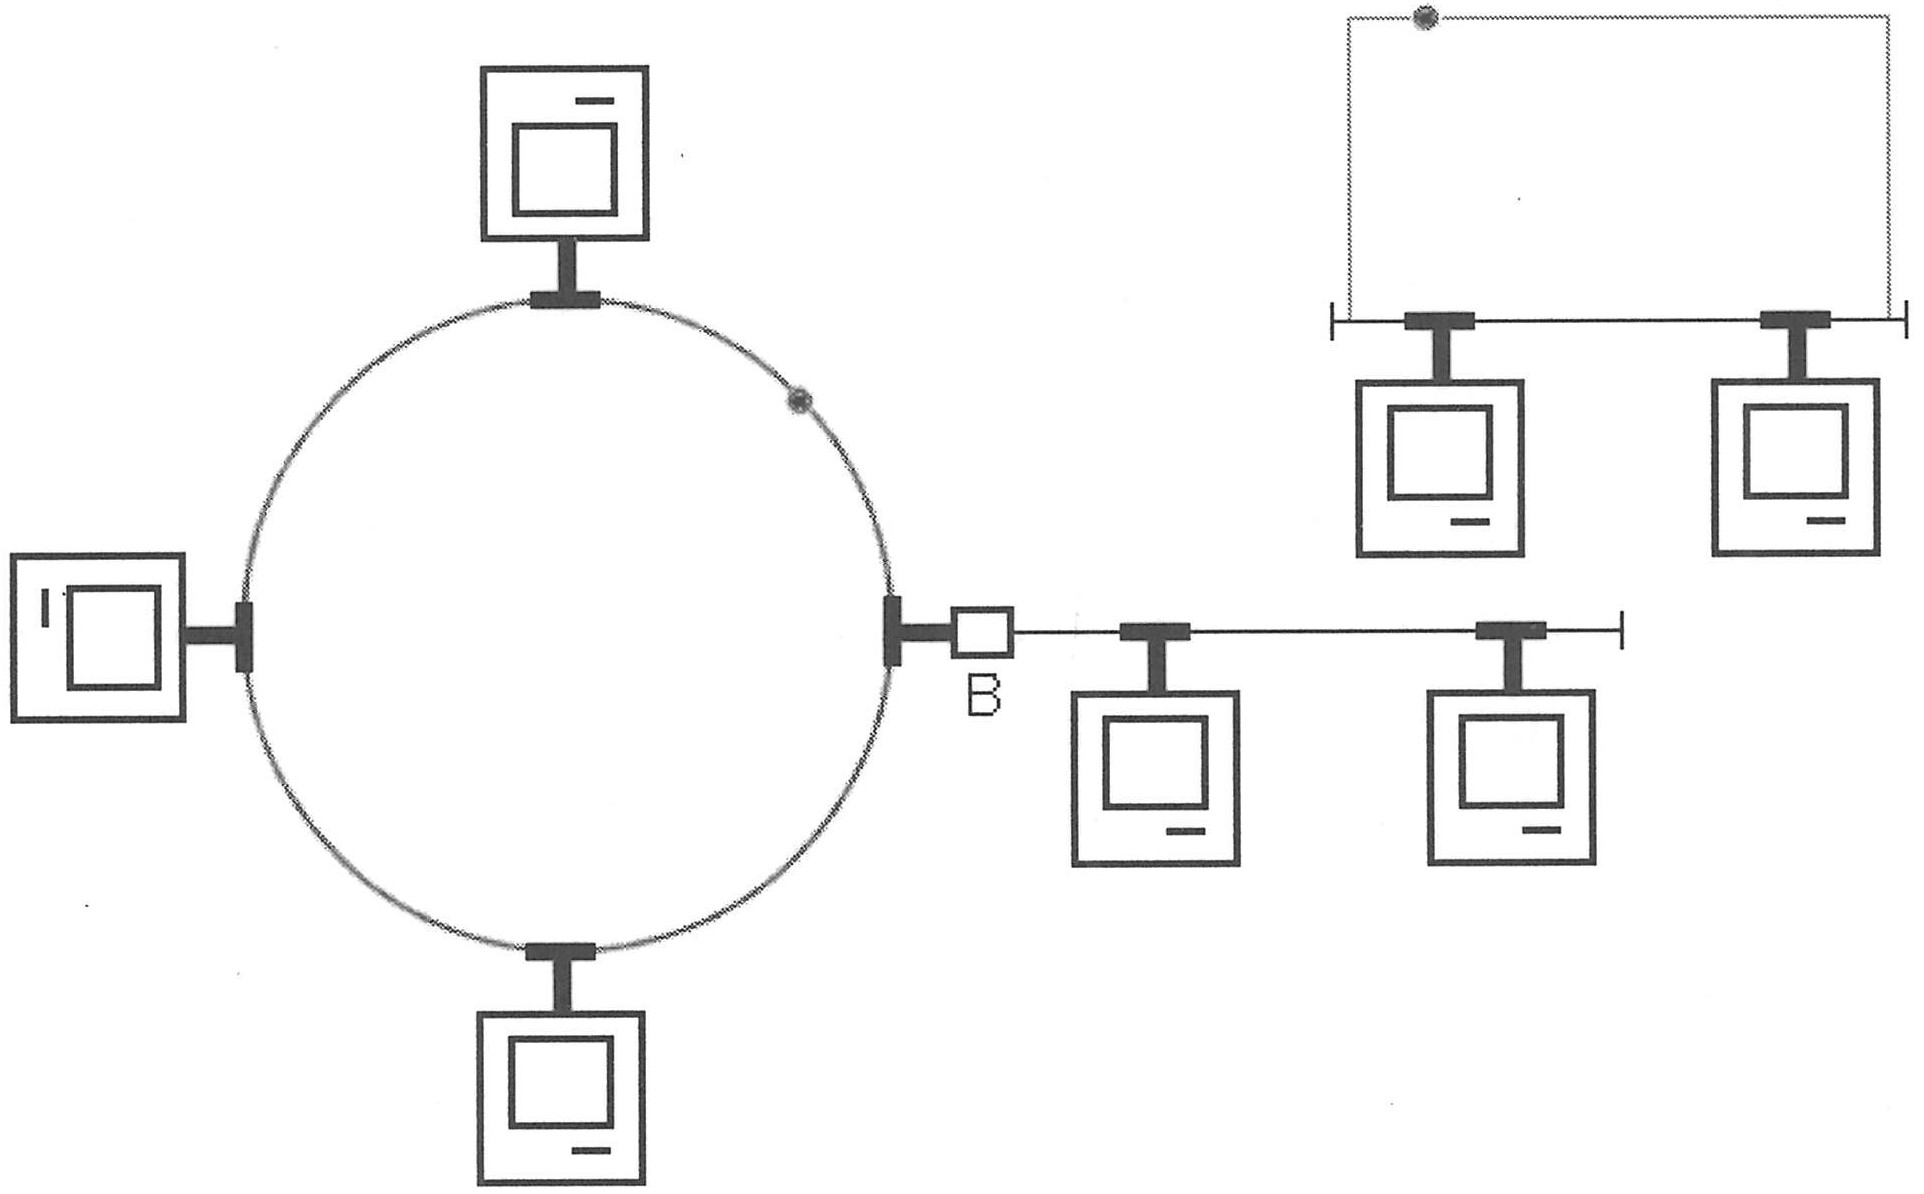
\includegraphics[width=\textwidth]{images/Token.jpg}
    \caption{Links: Token Ring. Rechts oben kleines Bild: Token wird auf einem Bus weitergereicht und am Ende wird es zum Anfang zurückgereicht und wieder gesendet.\cite{Schreiner2019}}
    \end{center}
\end{figure}

\subsection*{Was ist der Unterschied zwischen CSMA/CD und CSMA/CA? Wo werden sie verwendet?)}\label{sub:csma}\index{CSMA - Carrier Sense Multiple Access}
\textbf{CSMA: Carrier Sense Multiple Access}
\begin{itemize}
    \item Sender hört den Datenverkehr auf der Leitung ab (= carrier sense)
    \item Sender wartet, bis der Kanal frei ist
    \item sobald der Kanal frei ist, darf gesendet werden
    \item falls mehrere Sender (fast) gleichzeitig anfangen zu senden:\\Kollision $\rightarrow$ Wiederholung nach zufälliger Zeitspanne
\end{itemize}\,\\

\textbf{CSMA/CA (CA = Collision Avoidance)}
\begin{itemize}
    \item Kollisionsvermeidung durch zufällige Wartezeit nach Erkennung eines freien Kanals
    \item z.B. WLAN 802.11-DCF (Distributed Coordination Function)
\end{itemize}\,\\

\textbf{CSMA/CD (Collision Detection)}
\begin{itemize}
    \item sobald eine Kollision erkannt wird, wird die Übertragung abgebrochen
    \item z.B. Ethernet
\end{itemize}\,\\

\begin{tabularx}{\textwidth}{X|X}
    \multicolumn{1}{X}{CSMA/CD}&\multicolumn{1}{X}{CSMA/CA}\\
    \hline
    $\bullet$ Greift nach der Kollision&$\bullet$ Greift vor der Kollision\\
    $\bullet$ Genutzt in kabelgebundenen Netzwerken&$\bullet$ Genutzt in kabellosen Netzwerken\\
    $\bullet$ Reduziert die `'recovery time'' nach einer Kollision&$\bullet$ Minimiert Kollisionsgefahr\\
    $\bullet$ Bei Konflikt wird erneut gesendet&$\bullet$ Sendet zuerst die Info, dass etwas übermittelt wird\\
    $\bullet$ Effektiver als das einfache CSMA&$\bullet$ ähnlich effizient wie CSMA\\
\end{tabularx}

\subsection*{Was bedeutet „Late Collision“?}\index{Late Collision}
\begin{itemize}
    \item Definition:
    \begin{itemize}
        \item Late Collisions sind ein spezieller Typ von Kollisionen im Ethernet
        \item Kollision tritt nach den ersten 64 Bytes (512 bits) eines Frames auf (Mindestgrösse)
    \end{itemize}
    \item Ursachen:
    \begin{itemize}
        \item Ein wesentlich zu langes Netzwerkkabel
        \item Falsche Duplex-Einstellungen an Netzwerkkarte oder Switch
    \end{itemize}
\end{itemize}

\subsection*{Was muss man noch unbedingt über die physikalische Schicht und Zugriffsverfahren wissen?}
\begin{itemize}
    \item Übertragung nicht nur "`physisch"' per Kabel
    \begin{itemize}
        \item Schall
        \item Licht
        \item elektromagnetische Wellen
    \end{itemize}
    \item Geräte
    \begin{itemize}
        \item Hub
        \item Repeater
        \item Kabel
        \item Antennen
    \end{itemize}
\end{itemize}

\section{Antworten T2}
\subsection*{Was für Topologien findet man in Computernetzwerken?}
//TODO
\subsection*{Wo ist der Unterschied zwischen \flqq{}Bandwidth\frqq, \flqq{}Throughput\frqq{} und \flqq{}Goodput\frqq? Wie kann man diese Konzepte visualisieren und verstehen?}
//TODO
\subsection*{Was ist \flqq{}Latency\frqq{} und \flqq{}Jitter\frqq? Wie kann man diese Konzepte visualisieren und verstehen?}
//TODO
\subsection*{Was muss man noch unbedingt über Topologien und ``Bandwidth'' wissen?}
//TODO

\section{Antworten T3}
\subsection*{Was sind die wichtigsten Merkmale von Kupferkabeln?}
//TODO
\subsection*{Was für Kupferkabelarten werden heutzutage in Computernetzwerken am häufigsten verwendet?}
//TODO
\subsubsection*{Wie sind sie aufgebaut?}
//TODO
\subsubsection*{Wie sehen die Stecker aus?}
//TODO
\subsection*{Worauf muss bei der Handhabung und Verlegung der Kupferkabel besonders geachtet werden und warum?}
//TODO
\subsection*{Woraus resultieren die Längenbeschränkungen der Kupferverkabelung?}
//TODO
\subsection*{Was muss man noch unbedingt über Kupferkabel wissen?}
//TODO

\section{Antworten T4}
\subsection*{Was sind die wichtigsten Merkmale von Glasfaserkabeln?}
Glasfaserkabel haben eine Glasfaser als Übertragungsmedium und verwenden Licht, Laser oder UV als Übertragungsimpulse.

\subsubsection*{Wie sind sie aufgebaut?}
//TODO Bild

\subsubsection*{Wie sehen die Stecker aus?}
//TODO Bild

\subsection*{Worauf muss bei der Handhabung und Verlegung von Glasfaserkabeln besonders geachtet werden und warum?}
Glasfaserkabel sind zwar bis zu einem gewissen Rahmen biegbar, jedoch sollte der Biege-Radius nicht zu klein sein. Dies kann zu Reflexionen innerhalb der Node führen. Auf keinen Fall dürfen sie geknickt werden! Das Ende des Kabels muss stets mit einer Kappe geschützt werden.

\subsection*{Woraus resultieren die Längenbeschränkungen der Glasfaserkabelverkabelung?}
Wenn auch minim, so streut und absorbiert auch Glas das Licht (oder UV - Quarzglas). Mit der Distanz nimmt die Intensität des Lichts ab. Wie vorhin erwähnt, können Krümmungen zu Reflexionen führen, welche sich negativ auf die Übertragungsdistanz äusseren.

\subsection*{Wo ist der Unterschied zwischen Multi- und Singlemode (Monomode)- Glasfasern?}
//TODO

\subsection*{Was sind die Vor- und Nachteile von Glasfaserkabel (im Vergleich zu Kupferkabeln)?}
\begin{itemize}
    \item Vorteile
    \begin{itemize}
        \item unterstützt Bandbreiten bis zu 100 Gbit/s (im Labor über 1 Pbit)
        \item Entfernungen bis zu 100 km ohne Verstärker, über 1000 km mit Verstärker
        \item hohe Störfestigkeit gegen elektromagnetische Interferenzen
    \end{itemize}
    \item Nachteile
    \begin{itemize}
        \item hohe Kosten für Anschluss
        \item hohe Installationskenntnisse erforderlich
    \end{itemize}
\end{itemize}

\subsection*{Was muss man noch unbedingt über Glasfaserkabel wissen?}
//TODO

\section{Antworten T5}
\subsection*{Was sind die wichtigsten Merkmale von \flqq{}Wireless Media\frqq?}
//TODO
\subsection*{Welche Wireless Access Geräte arbeiten auf Layer I?}
//TODO
\subsection*{Was für Wireless Standards gibt’s in Computernetzwerken?}
//TODO
\subsubsection*{Was sind ihre Hauptmerkmale und Anwendungsbereiche?}
//TODO
\subsection*{Was sind die Vor- und Nachteile von \flqq{}Wireless Access\frqq{} Methoden im Vergleich mit \flqq{}Wired Access\frqq?}
//TODO